\documentclass[10pt,showpacs,preprintnumbers,footinbib,amsmath,amssymb,aps,prl,groupedaddress,superscriptaddress,showkeys]{revtex4-1}
\usepackage{graphicx}
\usepackage{dcolumn}
\usepackage{bm}
\usepackage[colorlinks=true,urlcolor=blue,citecolor=blue]{hyperref}
\usepackage{color}
\usepackage{algorithm}
\usepackage{hyperref}
\usepackage[noend]{algpseudocode}
\usepackage{mathtools}


\begin{document}

\section{Magneto-optical Trap Theory}
We use a one dimensional magneto-optical force derived in [1]:
\begin{equation}
\begin{multlined}
f_{MOT}(x, v_x) = - L \cdot (\beta x + k v_x) \\ 
L = \hbar k \Gamma\Delta\frac{\Omega^{2}/2}{(\Delta^{2}+(\Gamma/2)^{2}+\Omega^{2}/2)^{2})}
\end{multlined}
\end{equation}
Where $\Delta = \omega-\omega_{0}$, $\Omega = d \epsilon_{0} /\hbar$ is the Rabi frequency, $\Gamma$ is the decay rate, $\beta z$ is the zeeman term which accounts for an atoms resonant frequency shift due to the applied magnetic field, and $k v$ is the doppler term which accounts for the atom moving and thus shifting any received frequencies.
From this we consider an atom shifted off of the z axis. The laser follows a Gaussian beam profile, so we can tack on a normalized Gaussian to the force to account for the beam intensity:
\begin{equation}
F_{MOT}(x) = f(x,v_x)\cdot G(y,z)
\end{equation}
\begin{equation}
G(y,z) = \frac{e^{-(y^2/\sigma_{y}^2+z^2/\sigma_z^2)}}{2\pi\sqrt{\sigma_y\sigma_z}}
\end{equation}
In 3 dimensions, the total force is given by:
\begin{equation}
F_{MOT}(x,y,z) = f(x, v_{x})\cdot G(y,z)+f(y,v_{y})\cdot G(x,z)+f(z,v_{z})\cdot G(x,y)
\end{equation}
The potential for an atom moving along a path in the x direction is given by:
\begin{equation}
\begin{multlined}
U_{x} = -\int F_{MOT} \cdot dx \\
= L \cdot G(y,z) \cdot (\beta \int x \cdot dx +k \int v_x \cdot dx) 
= L \cdot G(y,z) \cdot (\beta x^2/2 +k v_x x)
\end{multlined}
\end{equation}

\begin{figure}[ht!]\label{2dpot}
  \centering
  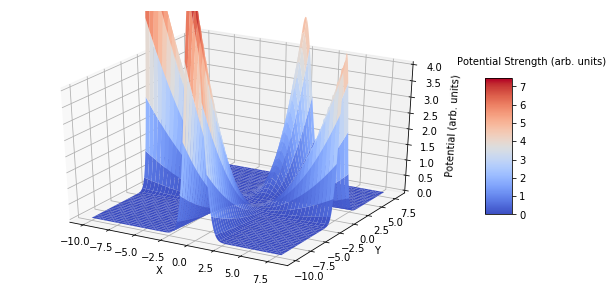
\includegraphics[width=0.5\textwidth]{/home/kristen/phy482/xy_zero_3d.png}
  \caption{The potential in 2-dimensions (x=0) for an atom with zero velocity. The repulsive portions are due to the laser beams whereas the well is where the atoms are classically trapped.}
\end{figure}
\begin{figure}[ht!]\label{2dpot_4}
  \centering
  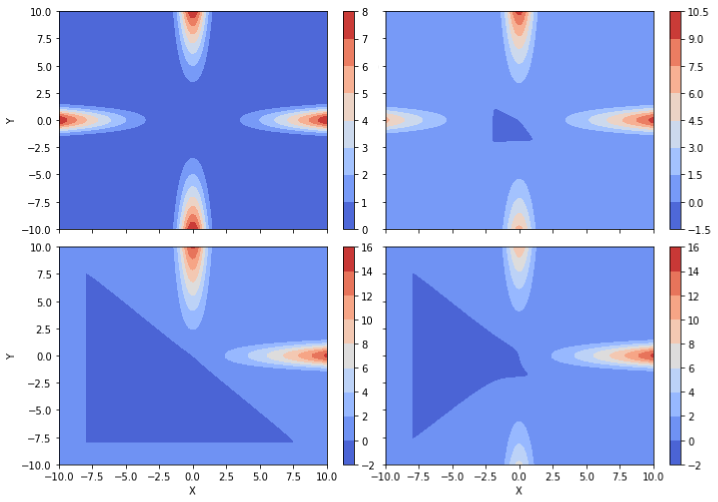
\includegraphics[width=0.6\textwidth]{/home/kristen/phy482/2d_potential.png}
  \caption{View of the potential in 2-dimensions for an atom with zero velocity (top left), positve 1 (arb. units) velocity in x and y directions (top right), positive 4 velocity in x and y directions (bottom left) and positive 4 velocity in x direction and positive 1 velocity in y direction (bottom right). The regions with minimum and maximum potential changes depending on the velocity of the atom. Larger velocities produce stronger repulsive potentials in the direction of motion and larger regions of potential wells opposite of the direction of motion.}
\end{figure}


In our future programs, we will have to discretize the velocity and the potential in order to show time dynamics.
\begin{equation}
\begin{multlined}
v_i = v_{i-1} + F_{MOT}(x_{i-1},y_{i-1},z_{i-1})t/m \\
t = t_{i}-t_{i-1}
\end{multlined}
\end{equation}


[1] http://www.iqst.ca/media/pdf/publications/PantitaPalittapongarnpim.pdf
\end{document}